\section{Experimental Methods}
\subsection{Photon Beam}
The accelerator's pulse width is set to 3 ns, where as the fastest and slowest neutrons in this experiment have a time of flight of 40 ns and 130 ns, respectively. A bremsstrahlung photon beam is produced by the passage of 10.5 MeV electrons through a 1" thick slab of aluminum. Aluminum was chosen as the radiator because it has a neutron knockout threshold above the energy of the 10.5 MeV electron beam. This prevents the bremsstrahlung radiator from being a source of fast neutrons, which could have the potential to travel into the experimental cell and cause false neutron events.

Downstream from the bremsstrahlung radiator, a sweeping magnet removes excess electrons from the photon beam (see figure~\ref{fig:Facility}). Before reaching the experimental cell, photons are collimated by a series of polyethylene and lead collimators aimed at eliminating beam contaminants.

** ToDo: Think about if/where to include the calculation of the ratio of knockout neutrons to fission neutrons. Have only done calculation for Thorium.  

When attempting a measurement of prompt neutrons from photofission, an ambiguity can arise between neutrons from photofission and neutrons from $(\gamma, xn)$. This is because the two reactions have similar cross-sections within the GDR region. Furthermore, there is significant overlap between the energy spectra of the neutrons from $(\gamma, xn)$ and photofission. Since this measurement is concerned only with observing two neutrons in coincidence, it suffices to set the Bremsstrahlung end-point at 10.5 MeV, since this value is below the threshold for ($\gamma, 2n$) of our targets ($\sim$12 MeV). Using an and-point of 10.5 MeV still leaves the possibility of the detection of multiple ($\gamma, 1n$) reactions in a single pulse, but this is an accidental coincidence. An \textit{accidental} neutron coincidence occurs when two uncorrelated neutrons happen to be detected in the same pulse. All accidentals follow Poissonian distribution, allowing for their subtraction from the data. The details of the procedure used to subtract accidentals is explained in section~\ref{Subtraction of Accidentals}.

The energy distribution of photons reaching the target was simulated using MCNP. The creation and collimation of the Bremsstrahlung photons in included in the simulation. The resulting energy distribution is shown in figure~\ref{fig:BremDist}

\begin{figure}[h]
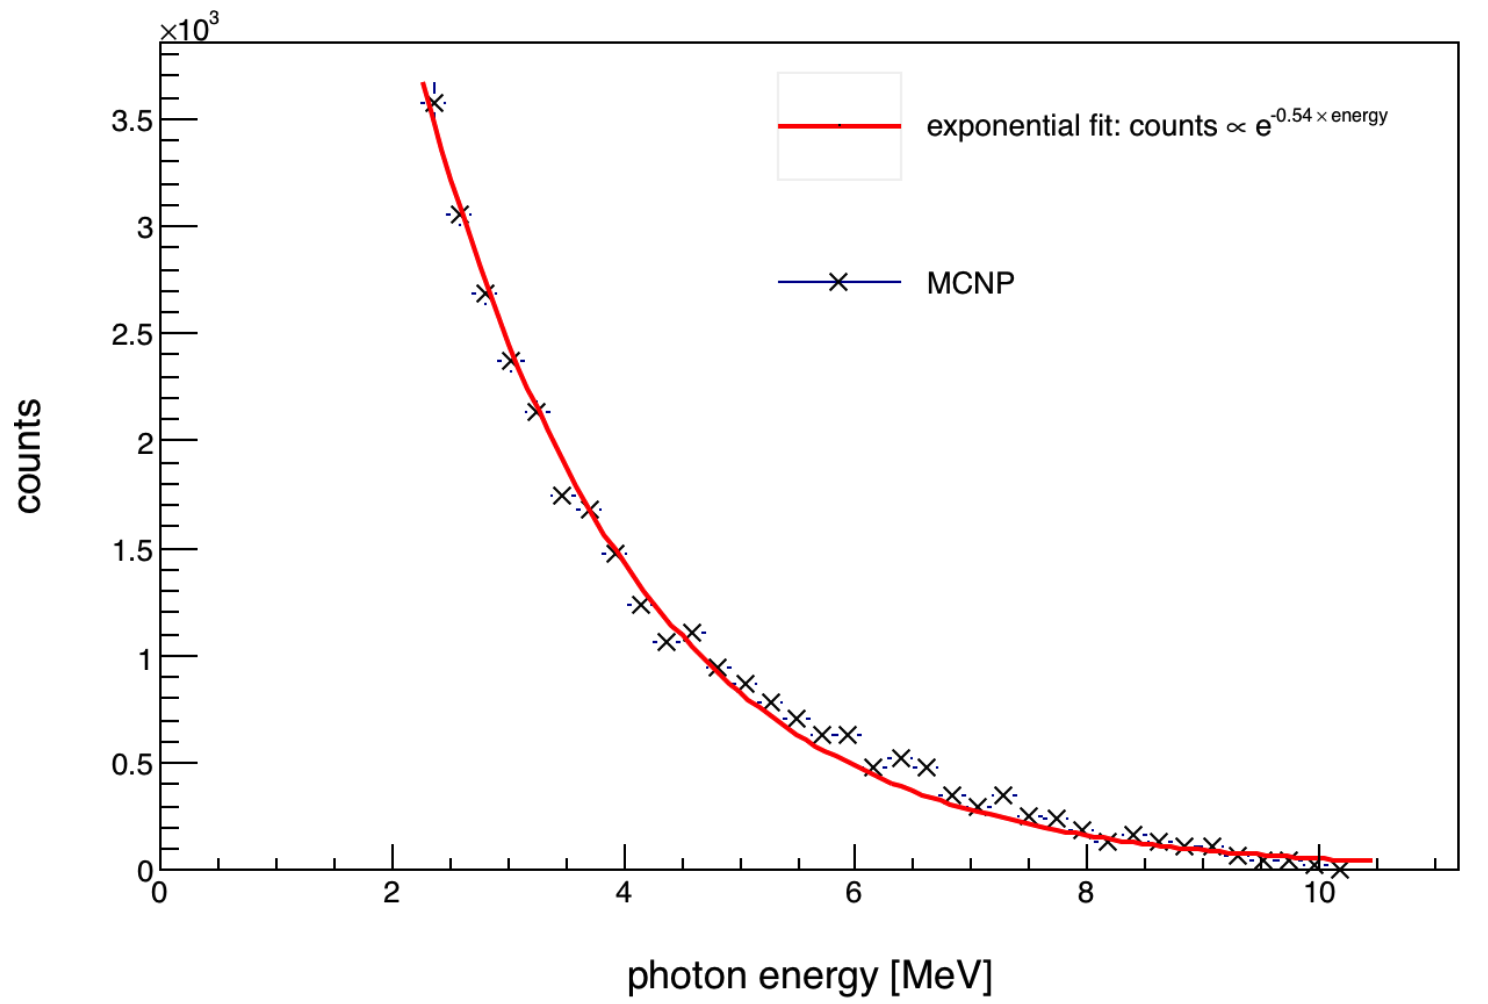
\includegraphics[width=0.9\textwidth]{Content/Methods/MCNPBremDistribution.png}
\caption{Result of an MCNP simulation of the energy distribution of the Bremsstrahlung photons that reach the target. Points are from the simulation, and the line is an exponential fit ($Ae^{-bx}$). The constant of proportionality, $A$, is arbitrary. The value for $b$ is 0.54.}
\label{fig:BremDist}
\end{figure}

The electron pulse width was set to 3 ns and had a 1.1A peak current, with a repetition rate of 240 Hz. The 3 ns pulse width was not a significant source of error in the measurements of neutron time of flight, since neutron events had a median time of flight of about 80 ns. 
The accelerator current is set by requiring there be, on average, fewer than one fission per pulse, thereby reducing the detection of uncorrelated neutrons from multiple fissions occurring in a single pulse. Even so, the detection of uncorrelated neutrons is unavoidable because of statistical fluctuations. To address this, a technique is developed to subtract these events from the data (see section~\ref{Subtraction of Accidentals}).

(Discussion about the LINAC's low duty factor??)

\subsection{Particle time of flight determination}
\label{reconstruction}

%python file: ProductionAnalysis/TOFGraphs
\begin{figure}[htbp]
\begin{center}

\subfloat[$\Delta T$s with no target in place. ]{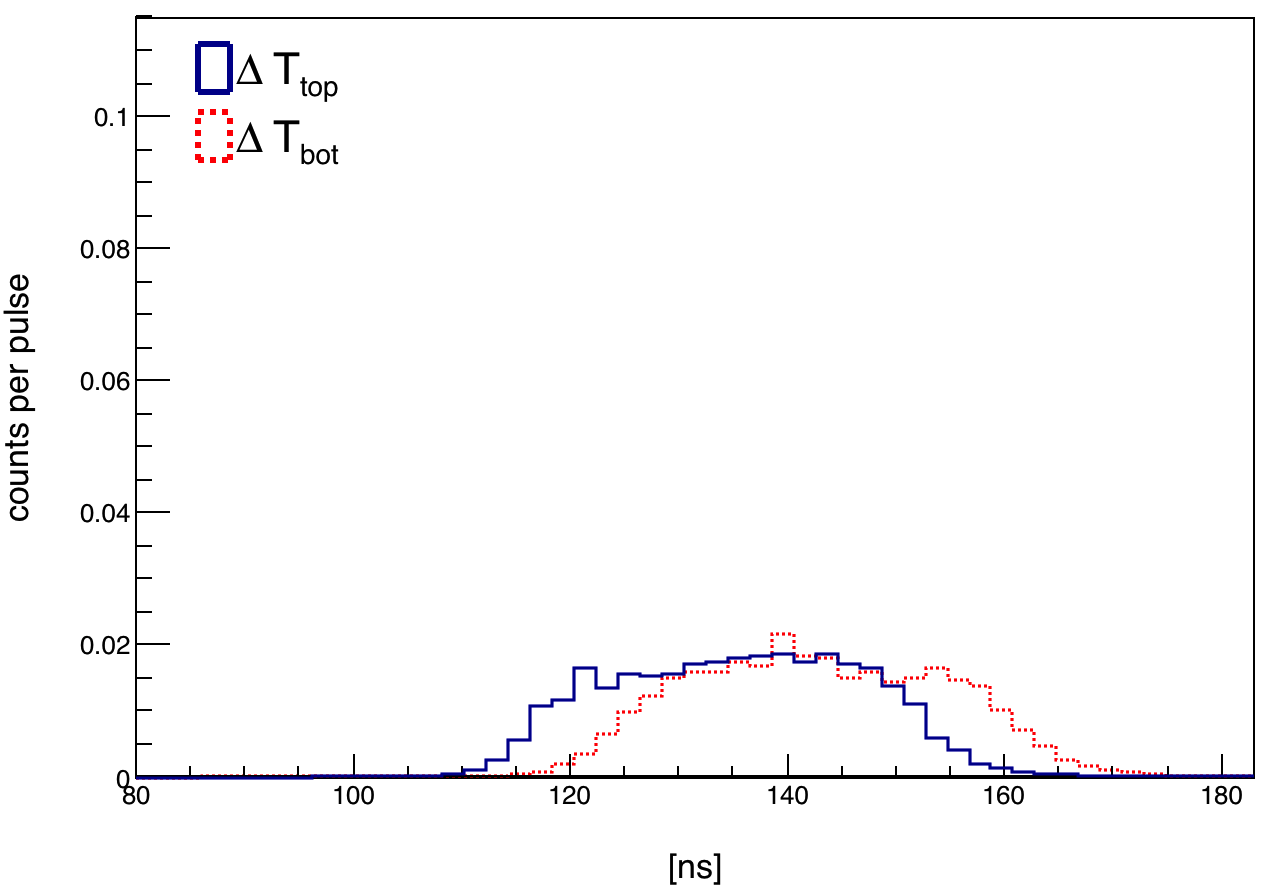
\includegraphics[width=0.5\textwidth]{Content/Methods/ToF0.png}}
\end{center}

\subfloat[$\Delta T$s with Aluminum target.]{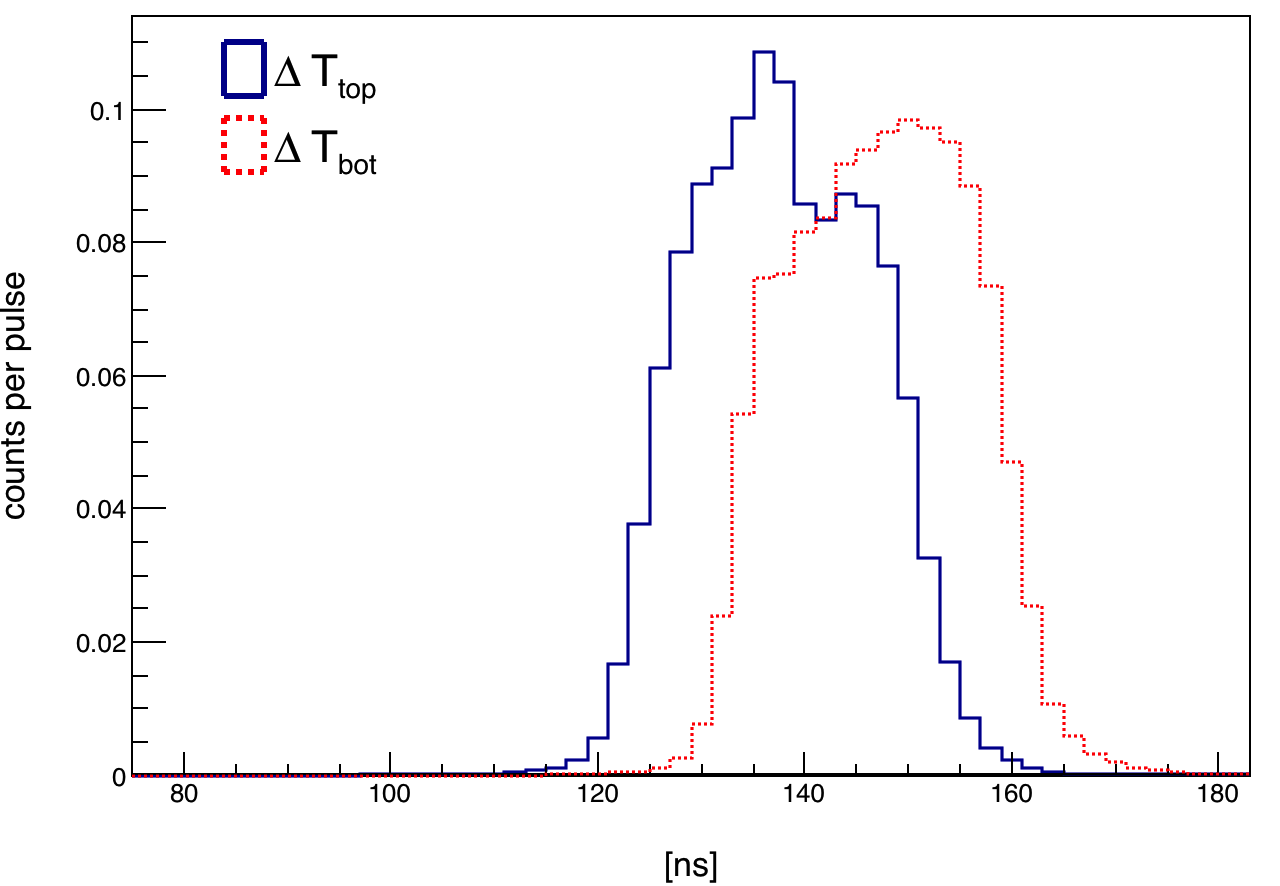
\includegraphics[width=0.5\textwidth]{Content/Methods/ToF1.png}}
\subfloat[Average of $\Delta T_{\text{top}}$ and $\Delta t_{\text{bot}}$  with Aluminum target in place.]{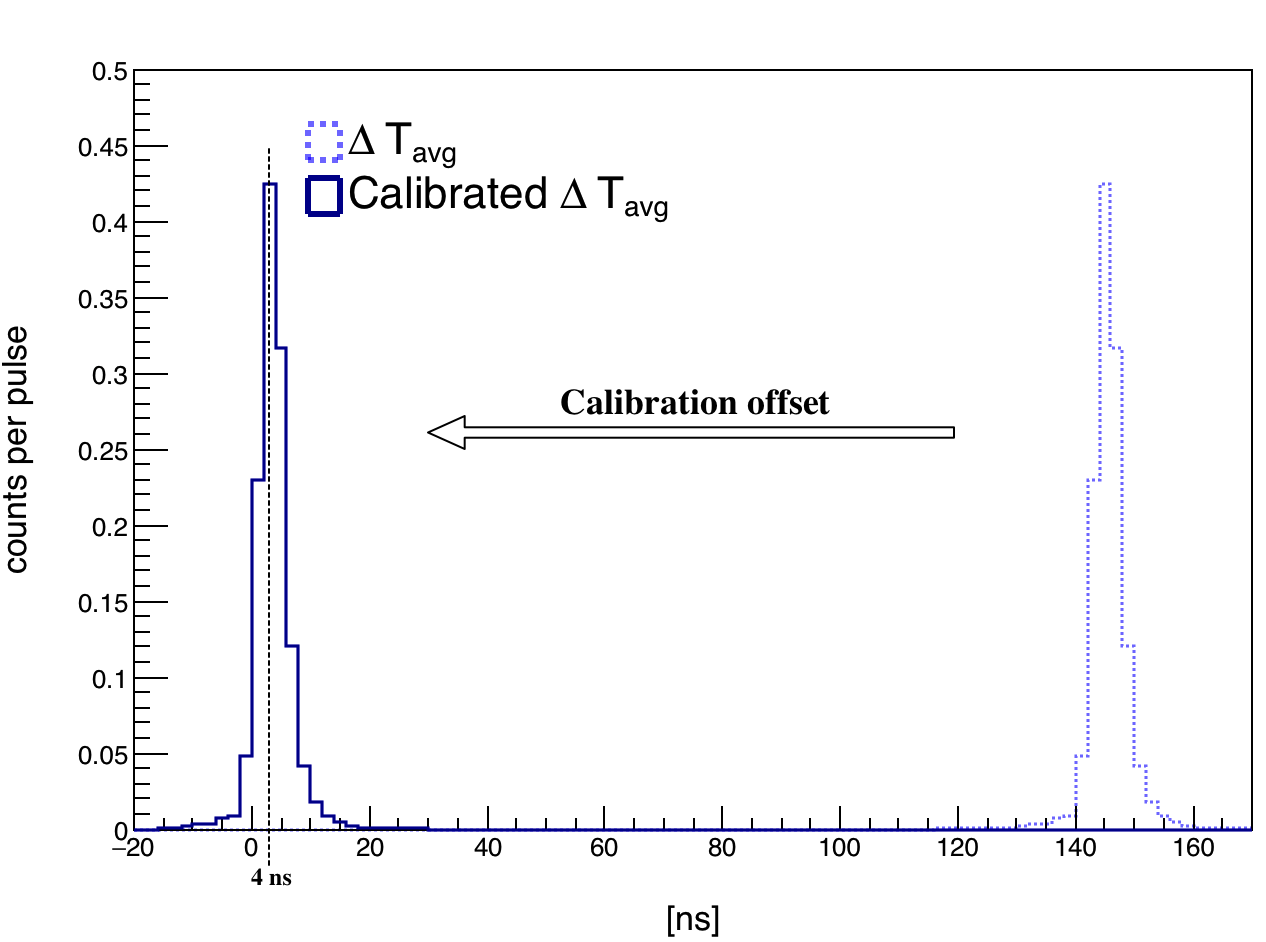
\includegraphics[width = 0.5\textwidth]{Content/Methods/ToF2.png}}
\caption{The $\Delta T $ spectra of PMTs with no target in place (a) shows the background produced by the beam alone. Using Aluminum as a non-neutron producing target (b), a peak appears in each spectra caused by photons scattering from the target. Since these photons travel a known distance of 1.25 m between the target and detector face, the width of these spectra reflect the range in scintillation light propagation times along the 76.2 cm length of the detector. Taking the average of the $\Delta T$s of the top and bottom PMTs produces a sharp peak (c), since the sum of the scintillation light propagation times from both PMTs is always equal to the time required for light to travel the detector's full length. The correct timing offset can be then be found using using the fact that photons have a time of flight of 4 ns. }
\label{fig:ToFDetermination}
\end{figure}

Each detector was equipped with two PMTs fixed on opposite ends of the scintillation cell, with the exception of the detectors located farthest downstream at $\pm30^{\circ}$, which only had a single PMT. The PMTs provide a signal in response to scintillation light with timing resolution of less than 1 ns. However, the main source of uncertainly in the time of a particle hit is variation in the time taken for scintillation light to propagate to the PMTs. No pulse shape discrimination was used in this study. Particle identification, along with the reconstruction of energy and position was achieved solely from the timing of signals from PMTs. The time of each event in a PMT was measured relative to a signal provided by the accelerator at the beginning of each pulse, which is referred to as the \textit{beam gun}.  

Time of flight (ToF), the time for a particle to travel from the target to the face of a detector, was used to distinguish between photons and neutrons, and to measure neutron energy. The time of flight was calculated by taking the average between the times of signals from the top and bottom PMTs, and subtracting an offset determined from a calibration. In the detectors located at $\pm30^{\circ}$, which have only one PMT, ToF is calculated from the timing of events in its sole PMT, minus a calibration offset.

The ToF of a particle that causes coincident events in both PMTs of a detector, obeys the following relationship:
\begin{displaymath}
ToF = C_i + \Delta t_{\text{avg}} 
\end{displaymath}
where $\Delta t_{\text{avg}} $ is the average between the timing from the top and bottom PMTs, and $C_i$ is a constant timing offset that is the same for every pulse. The subscript on $C_i$ is used because the timing offset is different for each detector. Any process that produces a timing delay that does not change from pulse to pulse contributes to $C_{i}$. Examples of this are the time required for photons to travel from the bremsstrahlung radiator to the target, the propagation of signals through the wires connecting the PMTs, and delays in the electronics for processing. 

The time required for scintillation light to travel through the detector, from point of scintillation to a PMT mounted at the detector's top or bottom, can vary from 1 ns for particles that hit very close to a given PMT, to about 8 ns for particles that hit across the detector from a given PMT. The sum of the times taken for scintillation light to travel to the top and bottom PMTs is just the time taken for the light to travel the full length of the detector, which is nearly constant. The rate at which light propagates along the length of a detector is dependant on speed of light in the material and the light's flight path. The flight paths of detected scintillation light tend to be parallel to the long axis of the detector, because these paths are the shortest possible, and only the first signal from a PMT is accepted. Therefore, by taking the average of the times in the top and bottom PMT, the time required for scintillation light to propagate through the scintillator becomes a constant offset.

The validity of a constant scintillation light propagation time was verified experimentally using a $^{60}Co$ source. With the face of the scintillator covered with 2" thick bricks of lead shielding, the $^{60}Co$ source is placed against the lead at several locations along the length of the detector. The lead brick between the $^{60}Co$ source and the scintillator has a small hole drilled through it, giving the $^{60}Co$ a direct line of sight to a point on the face of the scintillator.  

**ToDo: Make a figure for the setup of the co60 calibration. 

\begin{figure}
    \centering
    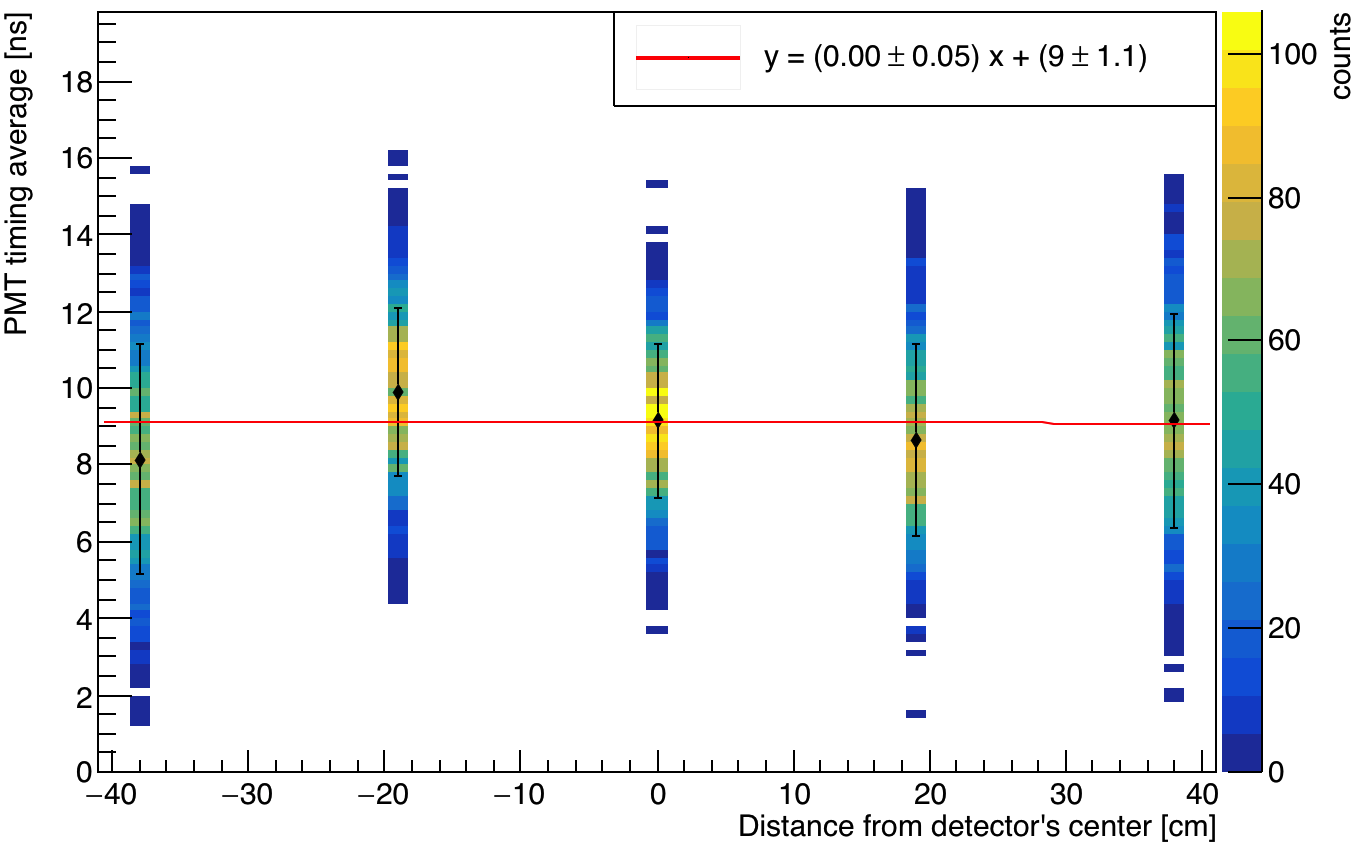
\includegraphics[width = 0.9\textwidth]{Content/Methods/CO60Validation.png}
    \caption{A $^{60}Co$ source, which emits coincident back-to-back photons, is placed at several positions along the face of a lead shielded scintillator. At each position, a small hole is drilled through the lead to give the $^{60}Co$ source a line-of-sight to a well-defined point on the scintillator. Then, a high timing resolution photon detector is placed close to the $^{60}Co$ source. $^{60}Co$ decays to emit two photons simultaneously--one photon is detected by the high timing resolution detector and serves as the ``start'' time, and the other photon causes a scintillation event in the detector being calibrated .}
    \label{fig:Co60Validation}
\end{figure}

\begin{figure}
    \centering
    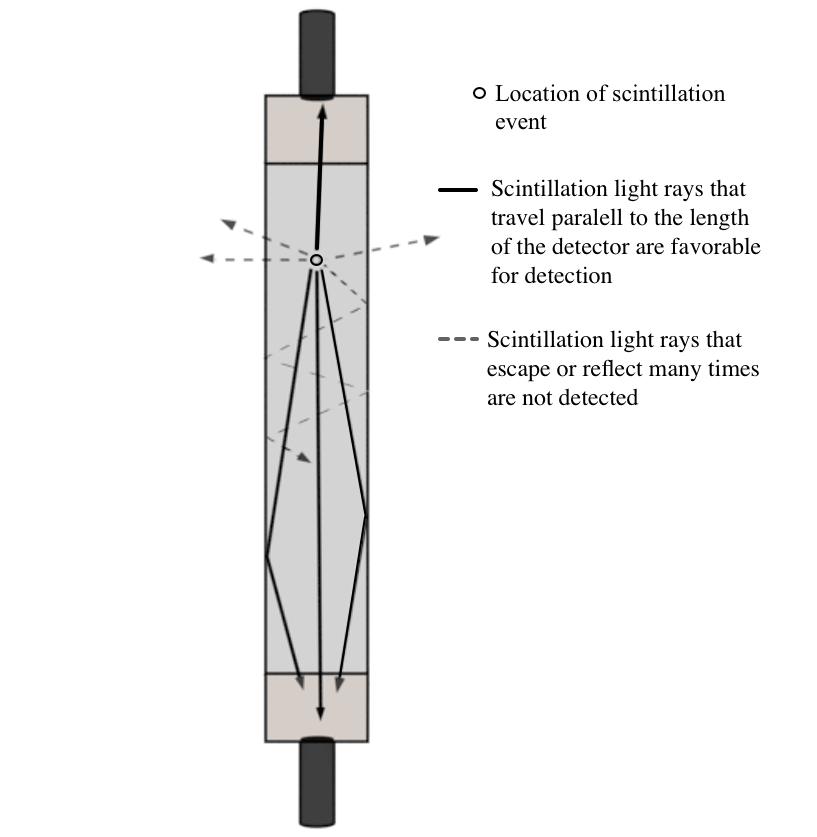
\includegraphics[width = 0.8\textwidth]{Content/Methods/lightpaths.png}
    
    \caption{Hypothetical paths of light rays as they propagate through the scintillator after a scintillation event. The light rays that first reach a PMT (solid) travel a shorter path than the others (dotted), and thus experience the least amount of attenuation. This experiment always uses the first signal from a PMT and hence the data favors cases in which scintillation light travels a short path to a PMT. In other words, the detectors favor the detection of scintillation light that is traveling parallel to the long axis of the detector. As a result, the sum of the times required for scintillation light to reach both PMTs is just the time taken for light to travel the full length of the detector, which is a constant. Thus, by taking the average time between coincident events in both PMTs, the time required for the propagation of scintillation light becomes a constant that is removed during calibration. 
    ** ToDo: Consider removing this figure :( }
    \label{fig:lightpath}
\end{figure}

The value of the constant offset for the calculation of ToF is determined by observing photons that are known to have scattered from the target. Comparing the timing spectra of a non neutron producing target made from aluminum, to the spectra produced when no target is used reveals a prominent peak caused by the photons that scatter from the target. The distance these photons must travel to reach the center of a face of any detector is 125 cm, and 130 cm to reach the top or bottom edges of a detector. It takes light 4.1 ns and 4.3 ns to travel 125 cm and 130 cm, respectively. The difference between these two ToFs is negligible compared to experimental uncertainty, so the ToF of photons that scatter from the target is assumed to be 4 ns, and with this assumption the constant timing offset of each detector can be calculated.  
   
\subsection{Particle position reconstruction}
Spacial resolution in the horizontal plane is determined by the physical dimensions of the detector. It's dimensions in the horizontal plane are comparatively small being 3.8x15 cm$^2$, so it suffices to use the geometric center of the detector as the horizontal component of a detected particle's position. In doing this, a positional uncertainty of $\pm$7.5 cm is introduced, which in terms of an opening angle is $\pm4^{\circ}$. The final results of this work use an opening angle bin width of 20$^{\circ}$, so $\pm4^{\circ}$ is not large enough be a cause for concern. The largest contributor to uncertainty in the reconstruction of particle position is the position in vertical direction, which is determined by the timing difference between signals in the top and bottom PMTs. 

As is the case with ToF determination, particle position in the vertical direction relies on the timing of coincident signals from both the PMTs of a detector. If both of the signals are the result of the detection of scintillation light created by the same particle, then the timing difference between the signals obeys a linear relationship with respect to the position of the particle hit along the vertical axis of the detector. The z-coordinate will hereafter refer to a particle's position along the vertical axis, where $z=0$ corresponds to the geometric center of the detectors. 

As discussed before, detected scintillation light tends to take fairly direct paths to the PMTs, experiencing few reflections off the boundary of the scintillation cell. As a result, the timing difference between signals in the top and bottom PMTs is proportional to the difference in path lengths that the scintillation light must travel to reach each PMT, which is in turn proportional to the z-coordinate of the particle hit. The exact linear relationship is determined through calibration by using collimated photons from a $^{60}$Co source. The calibration consists of measuring the top-bottom timing difference with the source of collimated photons fixed at five different locations along the detectors length. The result is shown in figure~\ref{fig:PMTDifference}. The setup for calibration was discussed in section~\ref{reconstruction}.

\begin{figure}
    \centering
    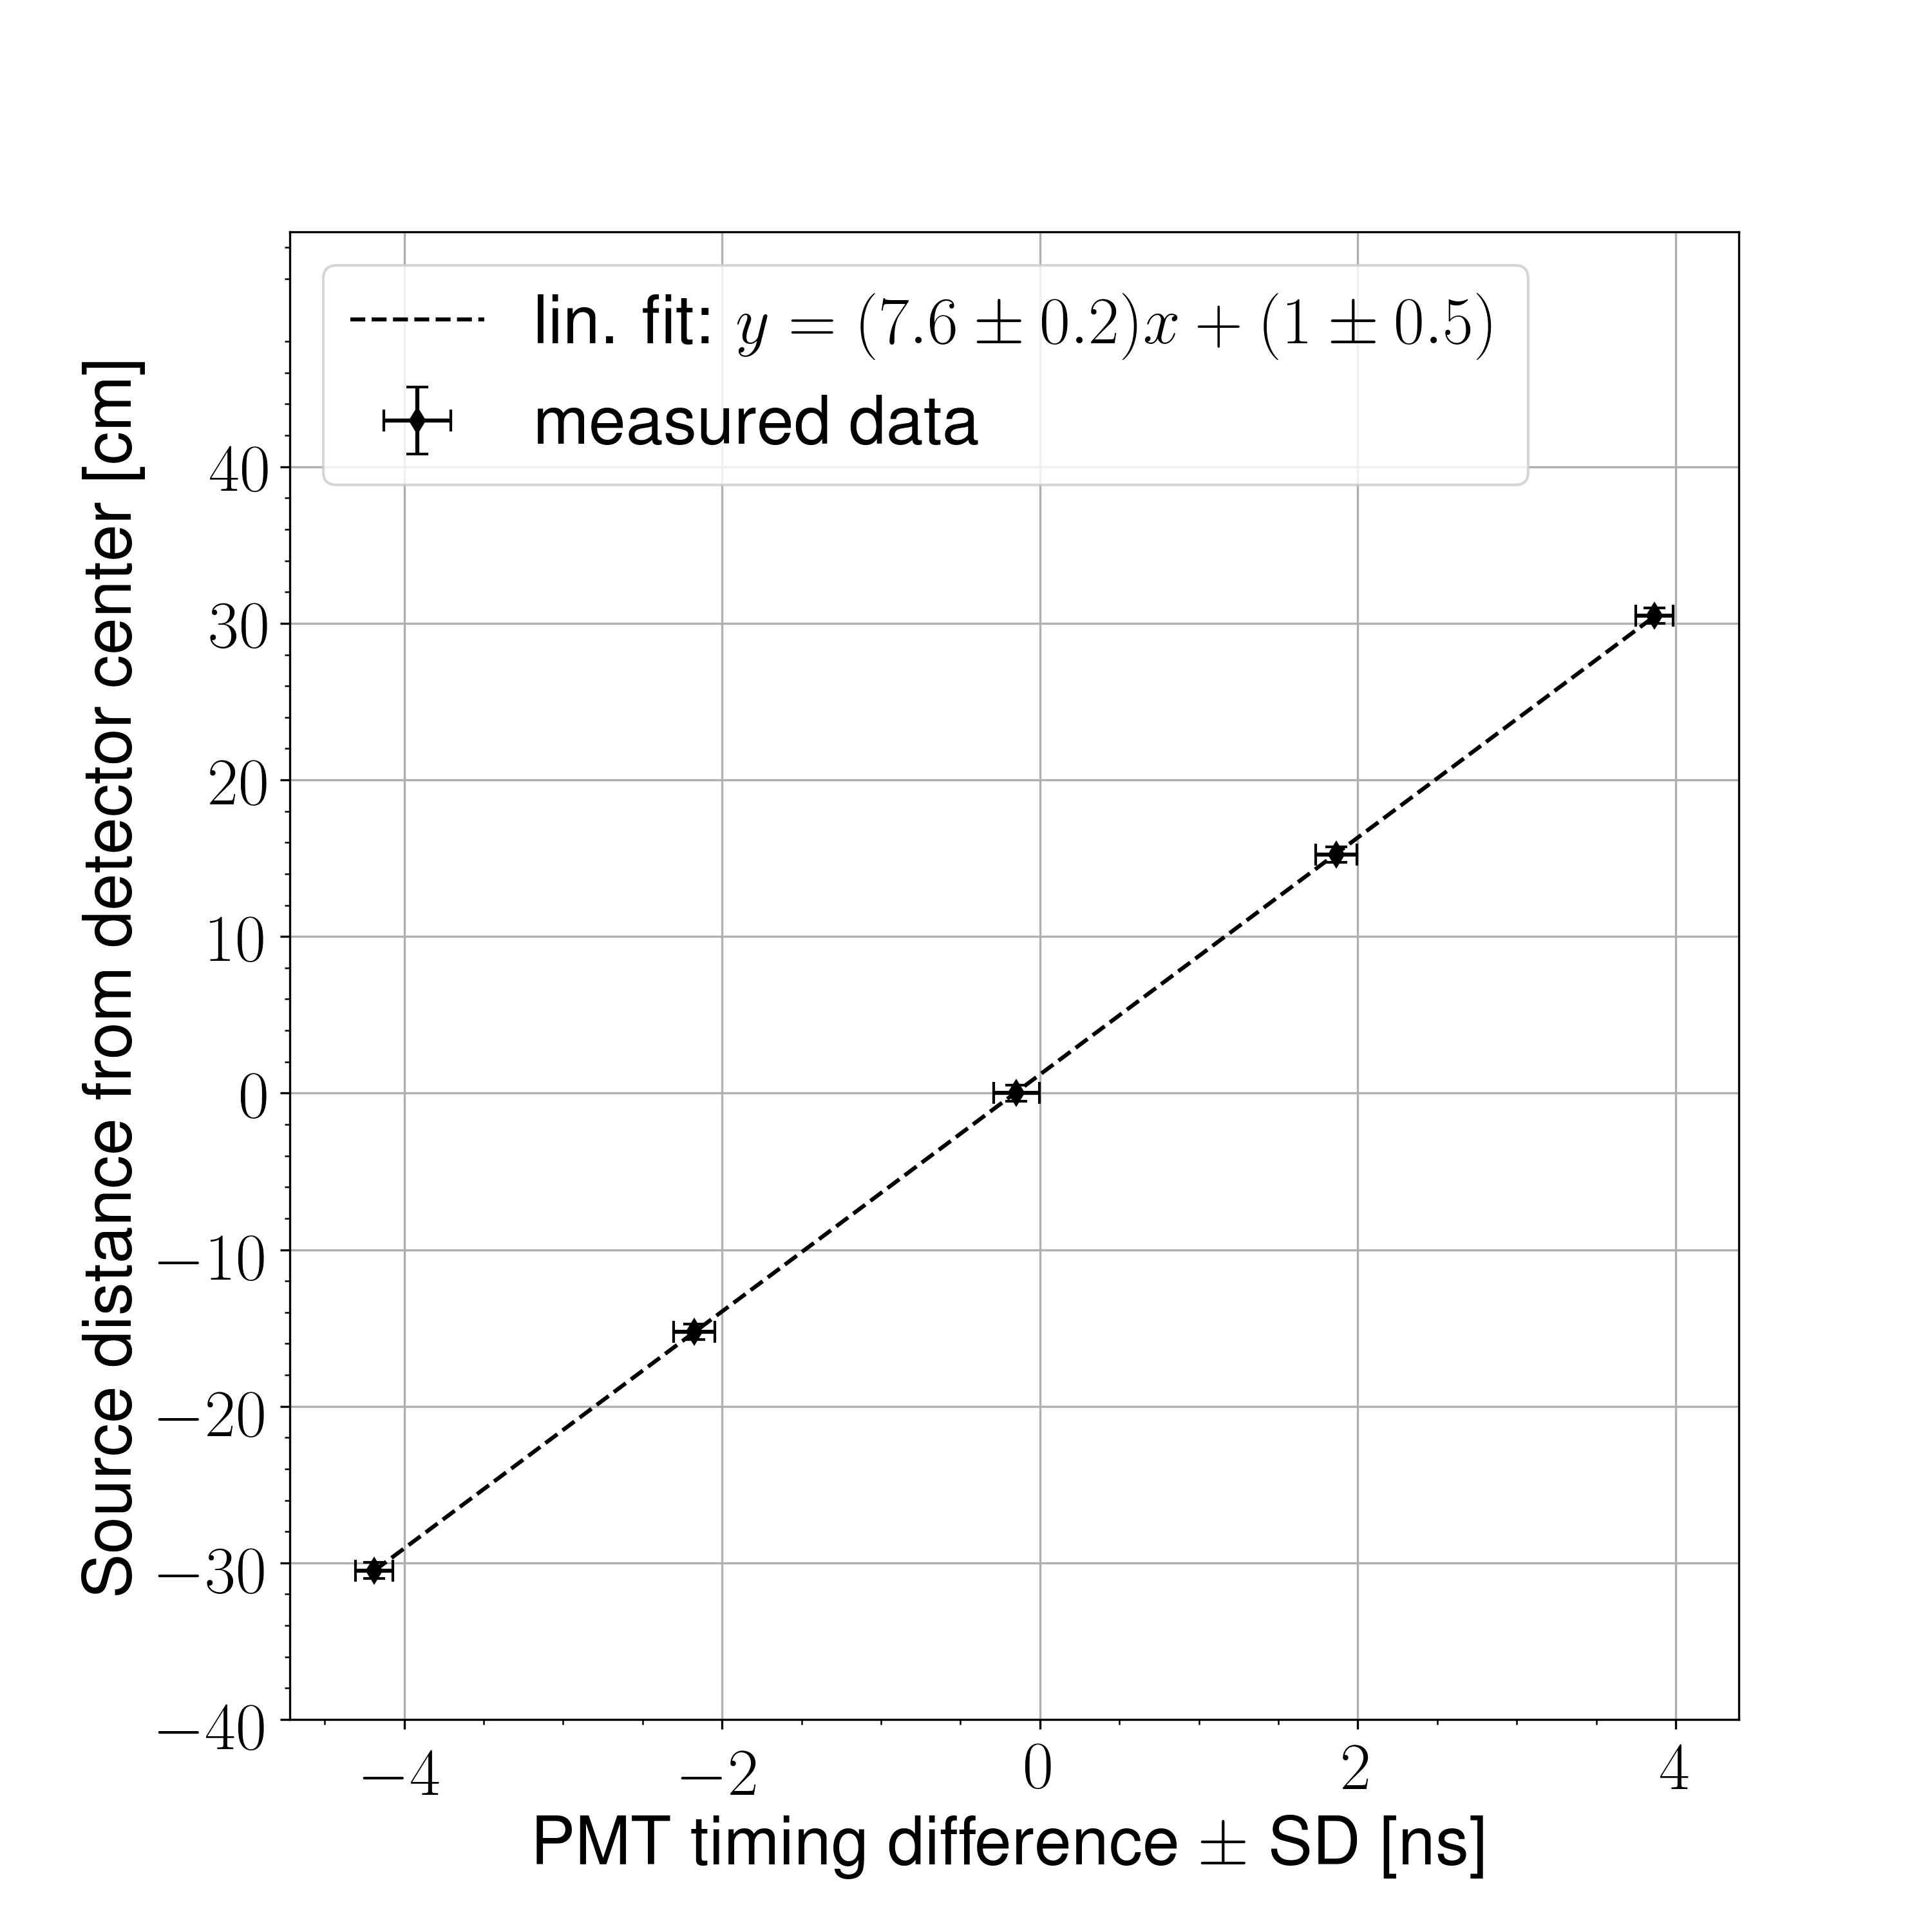
\includegraphics[width = 0.9\textwidth]{Content/Methods/PMTDifference.png}
    \caption{Using a collimated $^{60}Co$ source to produce events at a precise location on the detector, the particle's position along the detector's length is shown to vary linearly with respect to the timing difference between events in the top and bottom PMTs of a detector.}
    \label{fig:PMTDifference}
\end{figure}
\subsubsection{Detector Shielding}
** ToDo: Expand this section and add figures. 

The detector's shielding was designed with the aim of reducing cross-talk, the detection of photons, and noise. 
The front face of the detectors, which face towards the target, are subject to the highest flux of gammas due to scatting off the target. The detection of a gamma renders the detector ``dead'' during the time in which fission neutrons reach the detectors. Lead readily attenuates gammas, but has the side effect of causing neutrons to scatter and travel an unknown flight path to a detector, which destroys time of flight information. The extent that neutron flight paths are perturbed due to scattering in the lead shielding was quantified by an MCNP simulation. Accordingly, 1" of lead was placed along the front face of the detectors. This effectively diminished gamma detection rates and, according to the simulation, is expected to cause negligible levels of neutron scattering. Additional lead was used in some special areas that had high gamma flux: at the sides of detectors adjacent to the beam, and along the front faces of the detectors farthest downstream. 

Placing lead behind the detectors was avoided in consideration of an MCNP-POLIMI simulation, which indicated that lead placed here facilitates cross-talk. \textit{Cross-talk} is an undesirable phenomenon in which a particle causes a hit in one detector, and then by any means (e.g. scattering), the same particle causes a hit in a different detector. If both hits occur within the time frame typical for neutrons, then the cross-talk event cannot be distinguished from a true neutron coincidence. Because cross-talk events are in fact correlated, they cannot be removed in analysis by the subtraction of accidentals. 

\subsection{Detector Cross-talk}
**ToDo: Expand this section. Graphs and a more detailed discussion. The cross-talk plot on the wiki could be insightful. 

The geometry of the neutron detector array makes it kinematically impossible for a neutron to scatter from a proton--which is the basis for scintillation--only once within one detector, then travel directly to another detector without undergoing a second scattering event. Rather, it is kinematically required that a neutron must scatter from at least one intermediate nucleus before traveling into another detector. This fact can be derived from simple two-body kinematics. This kinematic requirement alone is not sufficient to neglect the occurrence of cross-talk, because the detectors and the shielding contain significant levels of carbon, lead, and other nuclei, which can function as intermediate scattering points. To address this, a detailed MCNP-POLIMI simulation was performed that modeled the entire neutron detector array, detector shielding and the supporting structures, and the experimental cell containing it all. Neutron detection physics was modeled to the point of neutron light output in MeVee, but did not include the propagation of scintillation light or its detection by the PMT tubes. A distinct feature of MCNP-POLIMI, which is not included in the standard MCNP release, is its ability to model a $^{252}$Cf spontaneous fission source that emits neutrons with the correct correlations.
The detection rate of correlated two-neutron events, relative to the rate of detected cross-talk events, is found by tracking fission neutrons individually through the geometry. In the simulation, coincident events were detected at a rate that is 36 times greater than for cross-talk events, which is less than a 3\% effect. Accordingly, no attempt was made to correct for cross-talk in the final result.


\subsection{Targets}
A depleted uranium (DU) target with dimensions of 4x2x0.0.05 $\text{cm}^3$ was used as the primary target for the measurement of two-neutron correlations. DU received the majority of the allotted beam time because it is an even-even nucleus, and as a consequence, has an anisotropic angular distribution of its fission fragments.

One consideration for the target dimensions is the rate of neutron scattering in the target. This has the potential to be a major problem, since a scattering event changes the neutron's direction of the travel and thus creates two-neutron opening angles that are not reflective of what the opening angle was immediately after fission. This effect cannot be eliminated completely, but the target must have small enough dimensions such that the effects of neutron scattering can be neglected. The probability that a two-neutron event is undisturbed by scattering is calculated by squaring the probability that a single neutron is not disturbed. The probability that a single neutron is not disturbed is calculated by an MCNP simulation in which neutrons with an energy spectrum typical of fission neutrons are sample uniformly within a target.

It is desirable to have a target with a symmetry that is consistent with the cylindrical symmetry of the neutron detector array. To accomplish this, a thin rectangular target was rotated slowly about the vertical axis during data acquisition. In doing so, cylindrical symmetry is preserved in the final result, since the final result is an average taken from events which occurred over a long period of time. 

\subsection{Elastic Scattering in Target}
**ToDo: Expand on this section. Discuss MCNP simulation and add a relevant plot. 

MCNP simulations indicated that the probability of a photo-neutron produced in the target escaped without scattering was 97.5\%. Because two neutrons are required for the formation of an opening angle, the rate of data contamination due to scattering is $(1-.975^2)$, or 5\% of two-neutron events.  


\subsection{Measurements with $^{252}$Cf}
**ToDo: reread this and revise. Maybe place result and comparison of Cf measurements here instead of in results?  

Opening angle measurements were also performed on neutrons from the spontaneous fission of $^{252}Cf$. The configuration for this measurement must be different than that for photofission measurements, as the photon beam can no longer be used as the timing ``start'' trigger. The trigger for $^{252}Cf$ consisted of two high timing resolution scintillation photon detectors, one fixed below and above the source at a distance of 15 cm. A 2-fold coincidence between both photon detectors, with a coincidence window of $\Delta t\leq 4$ ns, served as the timing start trigger. After a new start trigger is implemented, the analysis that follows is equivalent to that of photofission. 

As opposed to the measurement of neutrons from photofission, when using neutrons from $^{252}$Cf, there is no concern of accidental neutron pairs. Given the strength of the source, it is extremely unlikely for two fissions to occur during the neutron time of flight window, thus all detected neutron pairs are expected to be correlated. Another difference between the two measurements is the clean and sharp peak produced by fission photons from $^{252}$Cf, compared to the relatively smeared peak produced by photons scattering from the target during the photofission measurement. In both cases, the photon peak is used as a reference point for the time of flight of neutrons, so $^{252}$Cf has less error due to this effect. The normalization technique used in each case is the same, in which a correlated distribution is divided by an uncorrelated distribution. Because the opening angle distribution of neutrons from the spontaneous fission of $^{252}$Cf has been measured several several times with good agreement, its measurement in this study gives a good opportunity to verify the validity of the analysis techniques used.  
